\documentclass[fleqn, 14pt]{extarticlej}
\oddsidemargin=-1cm
\usepackage[dvipdfm]{graphicx}
\textwidth=18cm
\textheight=23cm
\topmargin=0cm
\headheight=1cm
\headsep=0cm
\footskip=1cm

\def\labelenumi{(\theenumi)}
\def\theenumii{\Alph{enumii}}
\def\theenumiii{(\alph{enumiii})}
\usepackage{comment}
\usepackage{indentfirst}
\begin{document}
%%%%%%%%%%%%%%%%%%%%%%%%%%%%
%% 表題
%%%%%%%%%%%%%%%%%%%%%%%%%%%%
\begin{center}
{\Large {\bf 作業発生の規則性を扱うカレンダシステムの評価の要約}}

\end{center}
\begin{flushright}
2013年 5月 8日

乃村研究室 河野 達生
\end{flushright}

\section{はじめに}
本資料は,作業発生の規則性を扱うカレンダシステムの評価[1]を読解し,要約したものである.

\section{情報処理学会研究報告『作業発生の規則性を扱うカレンダシステムの評価』要約}

\subsection{研究背景}
多くの作業はある程度決まった関連性と周期性にもとづいて発生している.本研究は,作業を行うときの関連性と周期性をモデル化し,評価することで,カレンダを将来の計画を支援する機能を備えたものとする研究である.次節では,モデルの詳細,および評価の観点について述べる.

\subsection{作業発生の規則性}
作業の発生には,ある程度決まった関連性と周期性がある.これを作業発生の規則性と呼ぶ.この関連性と周期性を扱うためのモデルを表現するため,以下の4つの用語を提案する.図1は,作業発生の規則性を適用した例である.
   \begin{enumerate}   		
	\item タスク(Task)\\
		タスクとは,作業を扱う最小の単位である.タスクは開始時間と終了時間を持ち,この間で連続的に行われる作業を表現する.
	\item リカーレンス(Recurrence)\\
		リカーレンスとは,タスク単位の周期性を扱うモデルである.リカーレンスは繰返し発生している同様のタスクを1つの集合とする.
	\item ミッション(Mission)\\
		ミッションとは,タスクまたはミッションを要素とするモデルである.ミッションはタスクまたはミッションを要素とし,複数の時間に分かれて実行される大きな粒度での作業を実現する.
	\item ジョブ(Job)\\
		ジョブとは,ミッション単位の周期性を扱うモデルである.ジョブは繰り返し発生しているミッションを1つの集合とする.
	\end{enumerate}

\begin{figure}[h]
  \begin{center}
    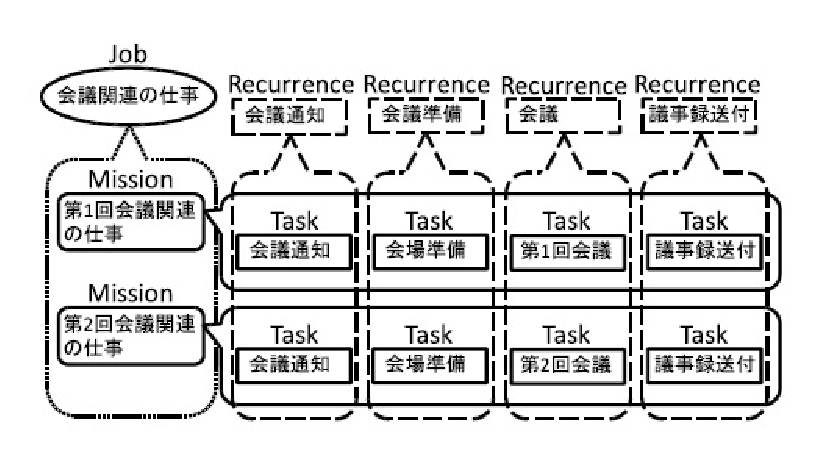
\includegraphics[clip,width=0.7\columnwidth]{zu4.eps}
    \caption{作業発生の規則性を適用した例}
  \end{center}
\end{figure}

	
リカーレンスを構成するタスクは,ある程度決まった周期性を持っていると考えられる.この周期性は,最後に発生したタスクと将来発生するタスクの間にも適用できると考えられる.これを\textgt{周期性の継承}と呼ぶ.また,繰り返し発生するタスクは,関連して発生するタスクもある程度決まっていると考えられる.この関連性は,将来発生するタスクにも適用できると考えられる.これを\textgt{関連性の継承}と呼ぶ.

\subsection{カレンダシステムを用いた計画立案}
既存のカレンダシステムは,過去の作業を振り返り,将来の計画立案を支援するには不十分であるといえる.対して,提案システムでは以下の3つの特徴により計画立案を支援する.
	\begin{enumerate}
		\item 過去のタスクを参照しながら複製するタスク登録方式\\
			1年前の同月のタスクを参照しながら,簡便な複製操作で当月のタスクを作成する登録方式である.
		\item 周期性の継承によるタスクの予報機能\\
			周期性の継承にもとづいて,近い将来発生しうるタスクを予測して提示する機能である.
		\item 関連性の継承による関連タスクの一括登録機能\\
			ミッション情報を利用して,ミッションに属する全タスクを将来の予定として展開して登録する機能である.
	\end{enumerate}

\subsection{評価}
\subsubsection{評価の方法}
カレンダシステムの3つの特徴によって,計画立案作業にかかる時間が,どの程度短縮されるかを評価する.以下の(評価1)と(評価2)を実施する.
	\begin{description}
		\item[(評価1)]本システムと既存のカレンダシステムで経過時間ごとの登録件数の変化を比較する.
		\item[(評価2)]本システムにおいて(特徴2)と(特徴3)を有効にした場合と無効にした場合で計画立案の初速を比較する.
	\end{description}
	
\subsubsection{評価の目的}
	\begin{enumerate}
		\item (評価1)の目的
		\begin{enumerate}
			\item 提案システム全体の総合的な効果を示す\\
				既存カレンダ(Googleカレンダ)との比較を実施する.
		\end{enumerate}
		\item (評価2)の目的
		\begin{enumerate}
			\item ユーザインタフェースの差の影響を排除する\\
				(評価1)では,ユーザインタフェースが作業発生の規則性を使った(特徴2),(特徴3)の有効性を端的に表すものではない.
			\item (特徴2),(特徴3)の効果をより詳細に調査する\\
	実際の立案作業は,ごく短い時間で実施するため,立案開始から短時間でも納得できる計画の立案が可能か否かが問題となる.この初速は,(特徴2)と(特徴3)の有効性の度合いを示しているといえる.したがって,特に計画立案の初期段階における効率を比較する.
		\end{enumerate}
	\end{enumerate}

% \subsubsection{実測評価}
\subsubsection{評価環境の準備}
実測評価の協力者はユーザAとユーザBの2名である.
2名には,過去2年間の予定を本カレンダシステムとGoogleカレンダの双方に登録してもらった.
本カレンダシステムでは,前年分についてリカーレンス,ミッション,およびジョブの関係を手動で与えてもらった.
過去2年間のタスク数を比較すると,ユーザBはユーザAの約2倍である.
また,ユーザBは,ミッション内に含まれるタスクが全体の約3分の1を占めている.
このことから,ユーザBのタスクは,複数のタスクが関連しながら発生している度合いが大きいユーザである.


\subsubsection{評価結果}
(評価1)と(評価2)の項目について評価結果を以下に記述する.
	\begin{enumerate}
		\item (評価1)の評価結果\\
%  過去の予定を再利用した計画立案速度\\		
実験協力者に時間無制限で次の1年間の計画立案をしてもらい,時間当たりのタスクの登録件数を測定した.測定の結果,Googleカレンダと比べて計画立案を効果的に支援できていると考えられる.この効果は(特徴1)の複製機能の影響が大きく,(特徴2)と(特徴3)はあまり影響していない.
		\item (評価2)の評価結果\\
%  作業発生の規則性を扱う効果\\
作業発生の規則性を扱うことによる効果を調べるため,計画立案の初期段階における初速を開始直後10分間について比較する.比較の結果,ユーザAは,長時間の考察を必要とせずにタスクを登録できている.予報機能により,再び発生するかどうかの手間が発生しなかったことが原因だと考えられる.しかし,過去の作業履歴に作業発生の規則性をあまり含まない場合,有用性は低くなる.
	\end{enumerate}
			
\section{まとめ}
今回は,作業発生のカレンダシステムについて理解するために,論文の要約を行った.論文の題材だけを研究するのではなく,研究を通してTODO管理ツールやタイムトラッカシステムの適用など研究の幅を広げることが重要だと感じた.
% 論文要約において,比較結果について理解できていないところが多く残った.


\begin{thebibliography}{99}
  \bibitem {book1} 三原俊介,谷口秀夫,乃村能成,南裕也:作業発生の規則性を扱うカレンダシステムの評価,研究報告マルチメディア通信と分散処理(DPS),Vol.2012-DPS-150,No.46,pp.1-6,(2012).\\
\end{thebibliography}

\end{document}
